\documentclass{article}
\usepackage{geometry}                		% See geometry.pdf to learn the layout options. There are lots.
\geometry{letterpaper}                   		% ... or a4paper or a5paper or ... 
%\usepackage[parfill]{parskip}    		% Activate to begin paragraphs with an empty line rather than an indent
\usepackage{graphicx}				% Use pdf, png, jpg, or eps§ with pdflatex; use eps in DVI mode
								% TeX will automatically convert eps --> pdf in pdflatex		
\usepackage{amsmath}
%\graphicspath{{/Users/lukebury/Documents/School/CU/ORCCA/}}
\usepackage{color}
\graphicspath{{../figures/}}

\usepackage[utf8]{inputenc} % allows for é

\newcommand{\paragraphtitle}[1]{\paragraph{#1}\mbox{}\\}

\title{Outline - APPM 5460 Proposal Outline}
\author{Luke Bury \& Don Kuettel}


\begin{document}
\maketitle


%=======================================================================================================
\subsection{Needs}
\begin{itemize}
  \item 2-4 pages
  \item Lit review
  \item dynamical system modeled by ordinary differential equations
  \item material from class\\\\\\
\end{itemize}

\subsection{Outline}
\begin{itemize}
	\item Intro (don)
	  \begin{itemize}
	  	\item In this proposal, we will be investigating homoclinic orbits in the Circular Restricted Three-Body Problem
	  	\item (tie to competition history)
	  	\item Homoclinic orbits are ... 
	  	\item They are important because ...
	  \end{itemize}
	\item History w/ Historical Lit Review (luke)
	  \begin{itemize}
	  	\item As documented by Andersson and Barrow-Green \cite{Andersson1994,BarrowGreen1994}, in 1885, Acta Mathematica announced a mathematics competition to the world. This competition, sponsored by King Oscar II of Sweden, encouraged interested parties to make an attempt at solving one of four selected problems.
	  	\item Henri Poincaré, a prominant mathematician of the time (who was largely favored to win the competition) chose to attempt the first problem, which essentially asked for a solution to the n-body problem. However, instead of the n-body problem, Poincaré decided to first attempt the three-body problem, since it was the first order of the problem that remained unsolved. To further simplify his initial effort, he restricted the three-body system in a manner known today as the Circularly Restricted Three Body Problem (CR3BP). 
	  	\item In the CR3BP, the origin is set at the barycenter of two bodies of interest (eg, Earth \& Moon), and the frame rotates so these bodies remain stationary on the x-axis. The bodies are assumed to move in perfectly circular orbits, and act as point masses from a gravitational perspective. The system is normalized so that the masses of the two bodies sum to 1 ($m_1 = \mu,\; m_2 = 1-\mu$), the distance between the bodies is 1, and the gravitational constant G is equal to 1. 
	  	\begin{figure}
	  	\centering
	  	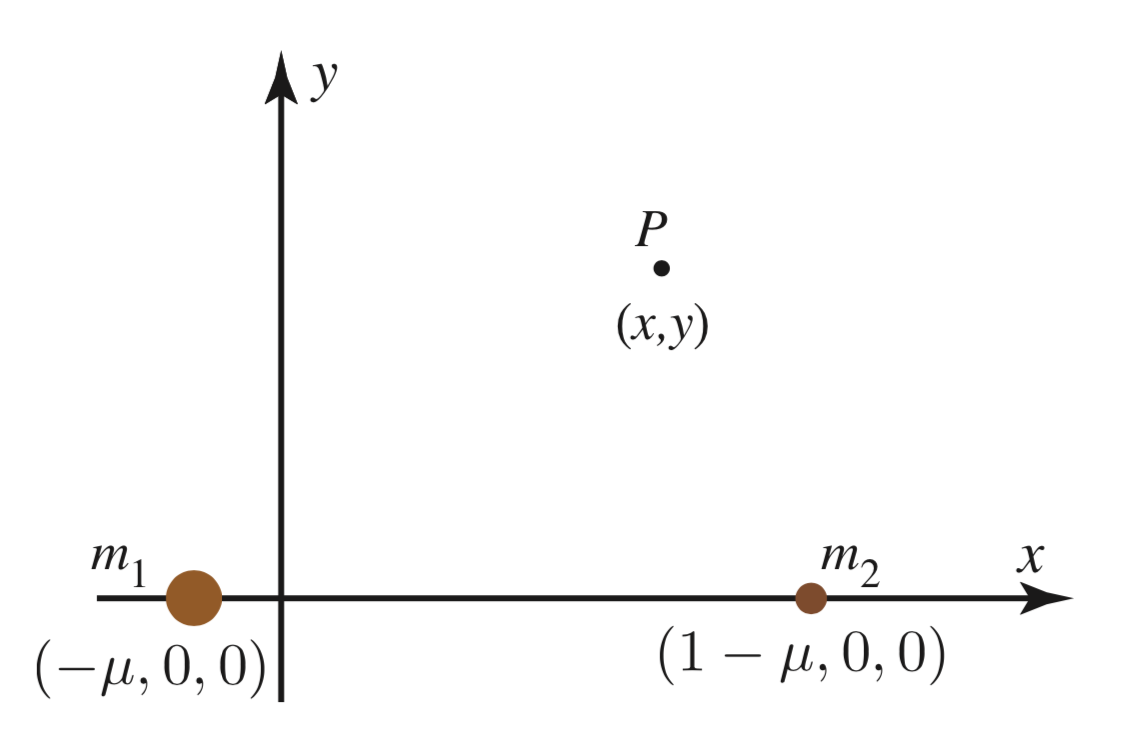
\includegraphics[scale=0.4]{CR3BP.png}\nonumber
	  	\caption{Layout of Circular Restricted Three Body Problem \cite{KoonLoMarsdenRoss2011}}
		\label{fig:CR3BP}
	  	\end{figure}
		\item Under these conditions, the equations of motion for the CR3BP are:
	  	\begin{align}
	  	\ddot{x} &=  2\dot{y} + x - (1-\mu)\left(\dfrac{x+\mu}{R_1^3}\right) - \mu\left(\dfrac{x-1+\mu}{R_2^3}\right)\\
		\ddot{y} &= - 2\dot{x} + y\left(-\dfrac{1-\mu}{R_1^3} - \dfrac{\mu}{R_2^3} + 1\right) \\
		\ddot{z} &= z\left(-\dfrac{1 - \mu}{R_1^3} - \dfrac{\mu}{R_2^3}\right)
		\end{align}
	  	%\item (a bit on the error ... discuss the math) ... as a result, discovered homoclinic points/orbits
	  	\item Poincaré submitted his work on the CR3BP, won the competition, and collected the prize. However, around the time of some of the first printings of his work, a discussion with Lars Edvard Phragmén led to the discovery of an error within Poincaré's submissiion that held significant ramifications.
	  	\item The error was rooted in Poincaré's failing "to take proper account of the exact geometric nature of a particular curve" \cite{BarrowGreen1997}. In Theorem III of the paper's first, and flawed, edition, Poincaré claimed that a particular invariant curve was closed (Figure \ref{fig:curveIntersection1}(a,b)). He failed to consider that the curve could be self-intersecting (Figure \ref{fig:curveIntersection1}(c)) - a mistake whose discovery cost him the fortune he had won, but also cemented his place among legendary mathematicians for his resulting discovery of \textit{doubly asymptotic}, or \textit{homoclinic}, trajectories.
	  	\begin{figure}
	  	\centering
	  	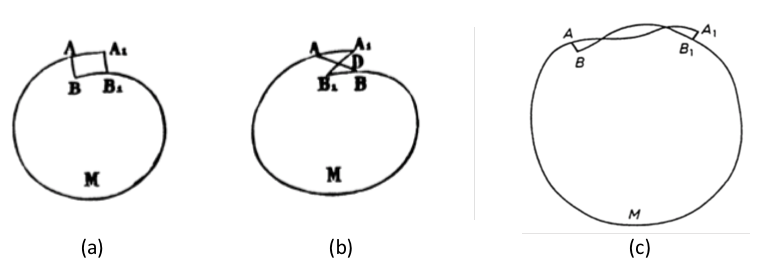
\includegraphics[scale=0.4]{curveIntersection1.png}\nonumber
	  	\caption{Invariant curve with self intersection from Poincaré's corrected work \cite{BarrowGreen1997}}
		\label{fig:curveIntersection1}
	  	\end{figure}

	  \end{itemize}
	\item Application w/ Modern Lit Review
	  \begin{itemize}
	  	\item \color{red}Much research has been conducted in this field since (references, references, references)\color{black}
	  	\item (pg 72+ of book)
	  	\item we will look at / recreate Poincaré's work
	  	\item we will create homoclinic orbits in the CR3BP using intersections of stable and unstable orbits in Poincaré plots
	  \end{itemize}
\end{itemize}

\bibliographystyle{plain}
\bibliography{../bibliography/appm5460.bib}

\end{document}  